\section{Circuito derivatore}
\begin{figure}[h]
	\centering
	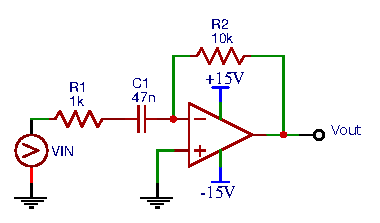
\includegraphics[scale=1]{derivatore.pdf}
	\caption{Circuito derivatore realizzato con l'opamp.}
	\label{f:derivatore}
\end{figure}
Si è montato il circuito in \ref{f:derivatore} con $R_1= \SI{0.981(9)}{\kohm}$, $R_2= \SI{9.87(9)}{\kohm}$,$C_1= 48\pm2$nF. Al variare della frequenza si è misurato $V_{out}$ con l'oscilloscopio, mantenendo l'ampiezza picco-picco di $V_{in}=\SI{2.08(2)}{\V}$. La frequenza è stata misurata con il frequenzimetro dell'oscilloscopio e lo sfasamento tra $V_{in}$ e $V_{out}$ si è ricavato dalla misura dell'intervallo di tempo $\Delta$T tra le due intersezioni delle onde in ingresso e uscita con l'asse delle ascisse \footnote{Tale asse orizzontale corrispomde per ogni onda ad una tensione costante pari al proprio valor medio}.Da questa misura si ricava lo sfasemento:$ \Delta\phi = 2\pi f\Delta T$.\\
Per quanto riguarda il guadagno in frequenza sono stati eseguiti due fit(in \ref{f:guad_deriv} e \ref{f:fase_deriv}), uno nella parte piatta dei dati cioè a basse frequenze ed un altro ad alte frequenze per studiare i due limiti del circuito derivatore, rispettivamente $f<<f_t$ e $f>>f_t$, dove  $f_t=\frac{1}{2\pi R_1C_1}= \SI{3.38(12)}{\Hz}$ è la frequenza di taglio. Si sono escluse le frequenze molto alte ($>\SI{50}{\kHz}$) poiché, avvicinandoci alla frequenza di taglio dell'opamp, i dati visibilmente non seguivano l'andamendo previsto per il circuito derivatore.

Ad alte frequenze ($f > \SI{13}{\kHz}$) è stato eseguito il fit di un valore costante, ottenendo il risultato :\\
$A_V= \SI{20.3 \pm 0.7}{\dB}$\\
$\chi^2=11.2 (4 \dof, p = 0.024)$\\
\\
A basse frequenze ($f< \SI{800}{\Hz}$) è stato eseguito il fit di  $A_V= m\log_{10} f/_{\si{\Hz}} +q$  e i risultati sono:\\
$m= \SI{-19.9(6)}{\dB\per\deca}$\\
$q= \SI{-50.0(11)}{\dB}$\\
$\chi^2=10.1 (8 \dof, p = 0.26)$\\
\\
Il valore atteso del guadagno ad alte frequenze è $A_V=20\log_{10} \frac{R_2}{R_1}= \ SI{20.1(2)}{dB}$ compatibile con il valore ottenuto dal fit.
A basse frequenze la pendenza della retta è compatibile con $\SI{-20}{\dB\per\deca}$.
L'alto $\chi^2$ per il fit dell'amplificazione costante è probabilmente dovuto al fatto che l'intervallo di frequenze su cui potevamo lavorare (quelle comprese tra le frequenze di taglio dell'opamp e del circuito derivatore) era troppo stretto perché si potesse effettivamente assumere che entrambi i due fattori vi restassero approssimativamente costanti; la distribuzione dei residui è un'ulteriore indicazione che questa potrebbe effettivamente essere la causa (sarebbe certamente spiegata da una curva di guadagno ancora concava anziché essenzialmente piatta).

L'intersezione della retta costante e della retta a \SI{-20}{\dB\per\deca} dà per $f_t$ un valore di \SI{3.34(4)}{\kHz}, compatibile con quanto previsto.

E' stato eseguito anche un fit dello sfasamento del segnale con la funzione $\Delta \phi= \arctan{\frac{f_t}{f}}$ e si è ottenuto:\\
$f_t= \SI{3.37(6)}{\kHz}$\\
$\chi^2=24.67 (12 \dof, p = 0.0164)$\\
Anche questo valore della frequenza di taglio risulta compatibile con quello atteso prima calcolato. L'alto $\chi^2$ è qua dovuto probabilmente agli errori sistematici (di cui non viene tenuto conto nel fit, poiché correlati tra i dati) sulle misure di $\Delta T$ a bassa frequenza, che teoricamente dovrebbero (qualunque siano le caratteristiche del circuito derivatore) dare un $\Delta \phi$ di $\pi/2\si{\rad}$ mentre sembrano invece nei nostri dati assestarsi su valori poco minori.

\begin{figure}[h]
	\centering
	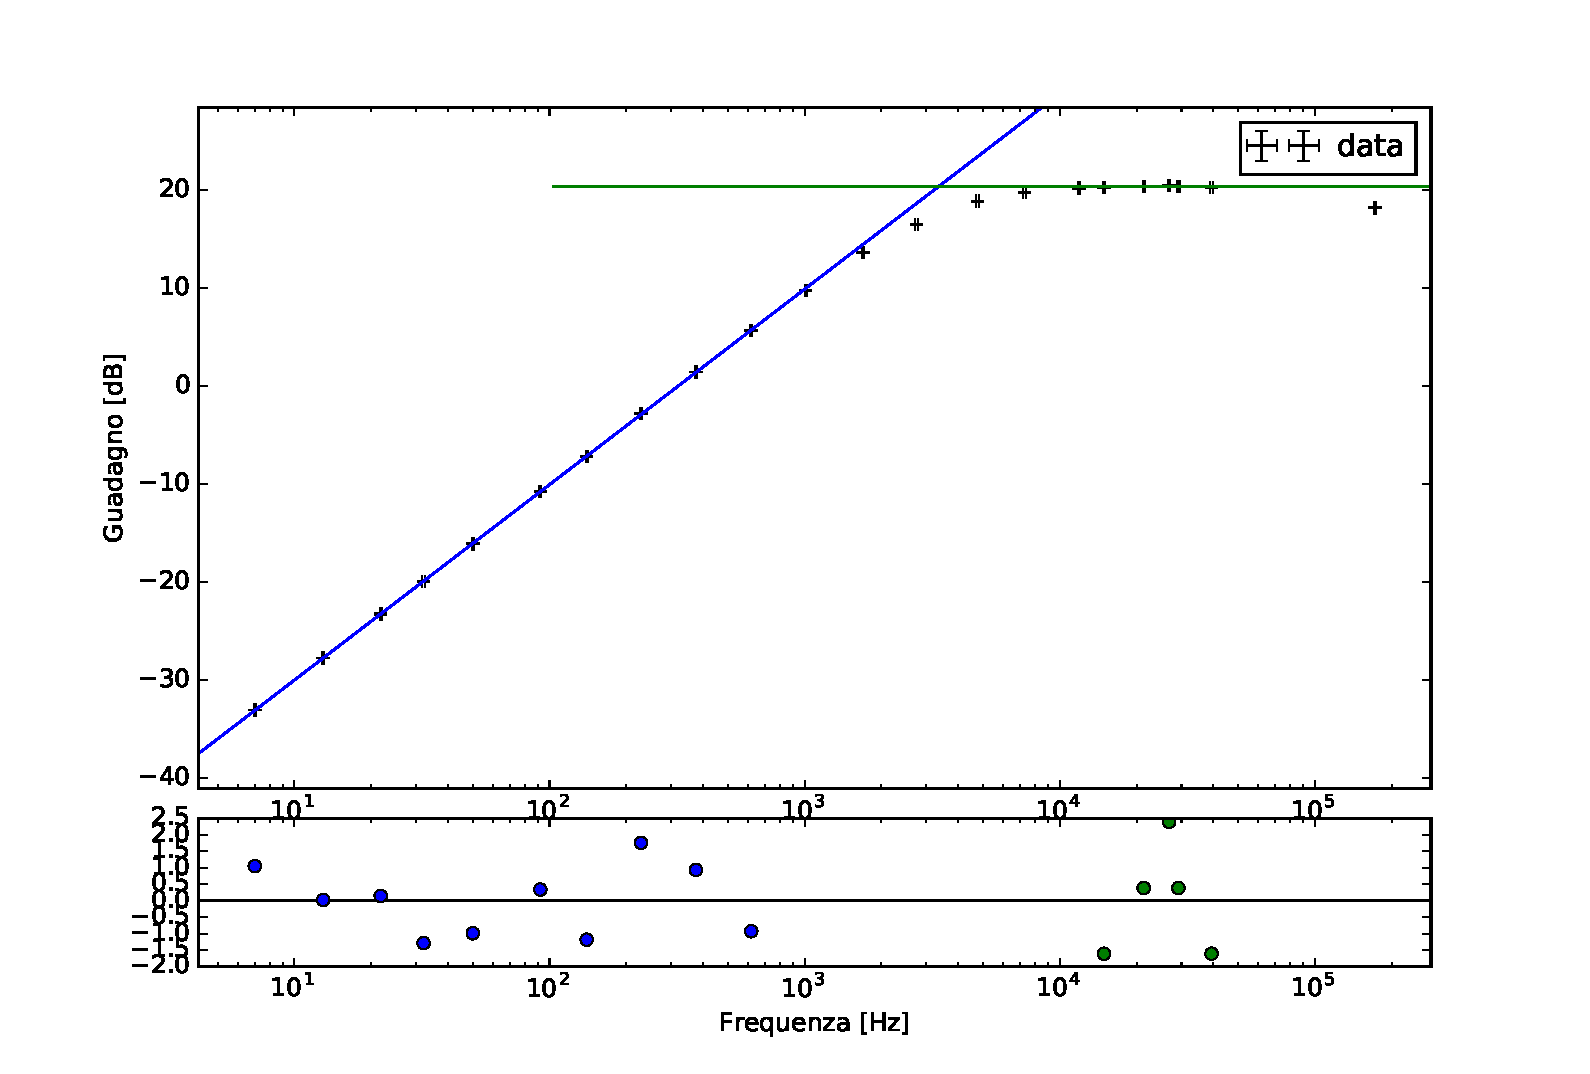
\includegraphics[scale=0.7]{fit_guad_derivatore.pdf}
	\caption{Bode plot del guadagno del circuito derivatore.}
	\label{f:guad_deriv}
\end{figure}

\begin{figure}[h]
	\centering
	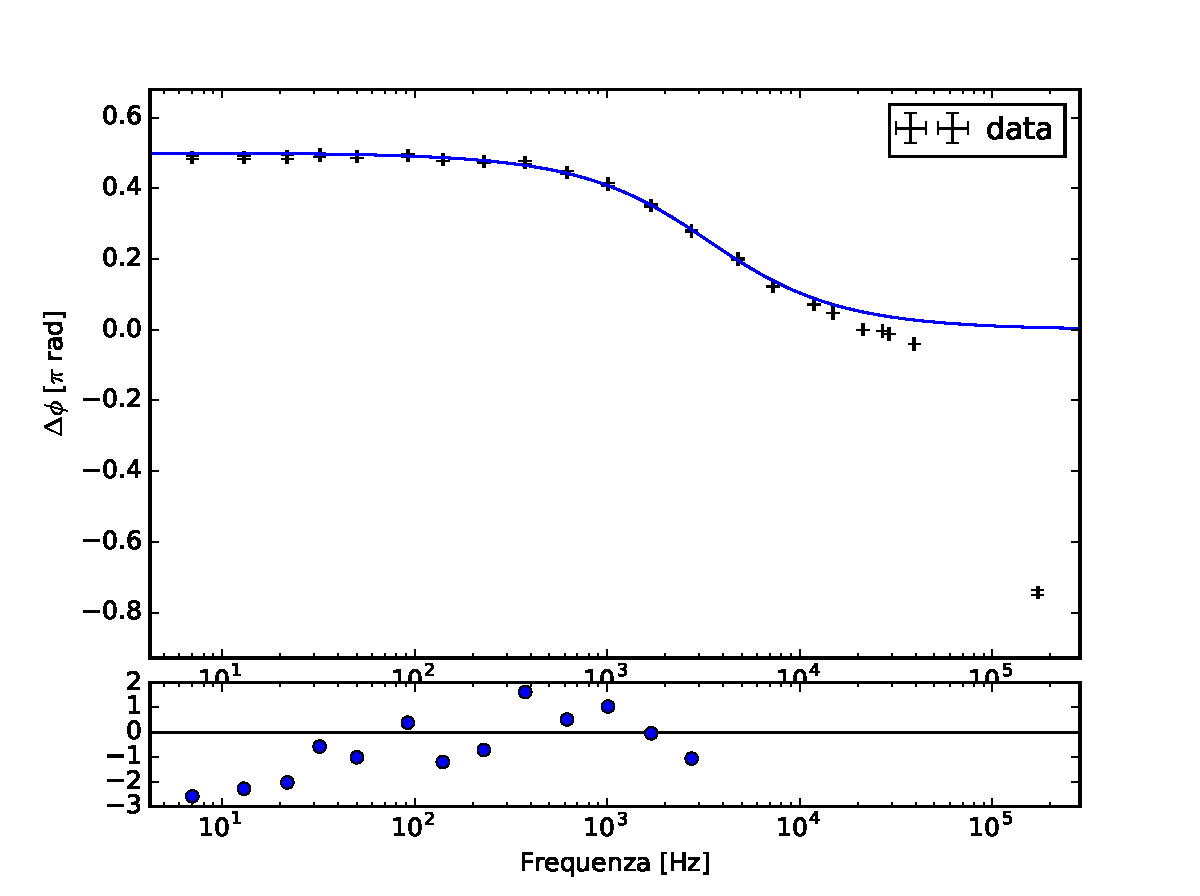
\includegraphics[scale=0.7]{fit_fase_derivatore.pdf}
	\caption{Sfasamento (in unità di $\pi\si{\rad}$) del circuito derivatore in funzione della frequenza.}
	\label{f:fase_deriv}
\end{figure}

Si è poi verificata la risposta del circuito ad un'onda triangolare di frequenza $f= \SI{97.87(15)}{\Hz}$. Con un'ampiezza di $V_{in}=\SI{2.26(5)}{\V}$ si è ottenuta un'ampiezza di $V_{out}=\SI{2.04(8)}{\V}$.

Dai grafici in \ref{f:deriv1}, in \ref{f:deriv2} e in \ref{f:deriv3} si nota che all'aumentare della frequenza (avvicinandocisi alla frequenza di taglio) l'output assomiglia sempre meno ad un'onda quadra, mentre a frequenze più basse la derivazione della triangolare in input sembrerebbe più regolare, ma visto il ridursi dell'ampiezza, il maggior impatto del rumore non permette di apprezzare gli eventuali miglioramenti sulla forma d'onda in uscita.
Il ruolo di $R_1$ è quello di stabilizzare il circuito derivatore riducendo il guadagno alle alte frequenze; ciò permette sia di controllare meglio il comportamento del circuito (eliminando l'influenza del comportamento caratteristico dell'opamp in saturazione) sia di evitare un'eccessiva amplificazione del rumore ad alta frequenza, che essendo sempre presente rischierebbe altrimenti di sovrastare il segnale (o quantomeno di essere sempre molto significativo). Analizzando il circuito in trasformata di Laplace, aggiungendo $R_1$ il polo della funzione di trasferimento passa da $s=oo$ a $s = -\frac{1}{R_2C_1}$: si rimuove la divergenza del guadagno per alte frequenze.


\begin{figure}
	\centering
	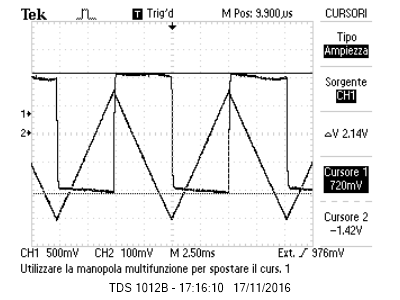
\includegraphics[scale=1]{data_derivatore1.png}
	\caption{Risposta derivatore ad un onda triangolare di frequenza $\SI{97.9}{\Hz}$.}
	\label{f:deriv1}
\end{figure}

\begin{figure}
	\centering
	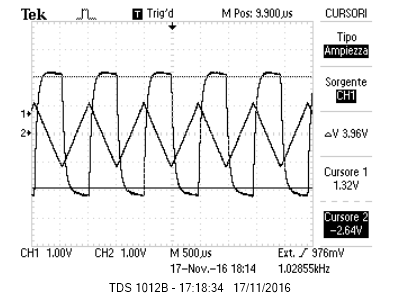
\includegraphics[scale=1]{data_derivatore2.png}
	\caption{Risposta derivatore ad un onda triangolare di frequenza $\SI{1.02}{\kHz}$.}
	\label{f:deriv2}
\end{figure}	

\begin{figure}
	\centering
	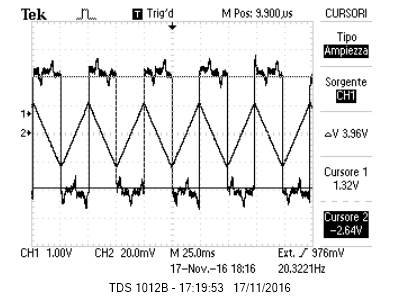
\includegraphics[scale=1]{data_derivatore3.png}
	\caption{Risposta derivatore ad un onda triangolare di frequenza $\SI{20.3}{\Hz}$.}
	\label{f:deriv3}
\end{figure}